\begin{figure}[h!]
\vspace*{-2ex}
\centering
%\setlength{\tabcolsep}{3pt} % Default value: 6pt
%\renewcommand{\arraystretch}{0.5} % Default value: 1


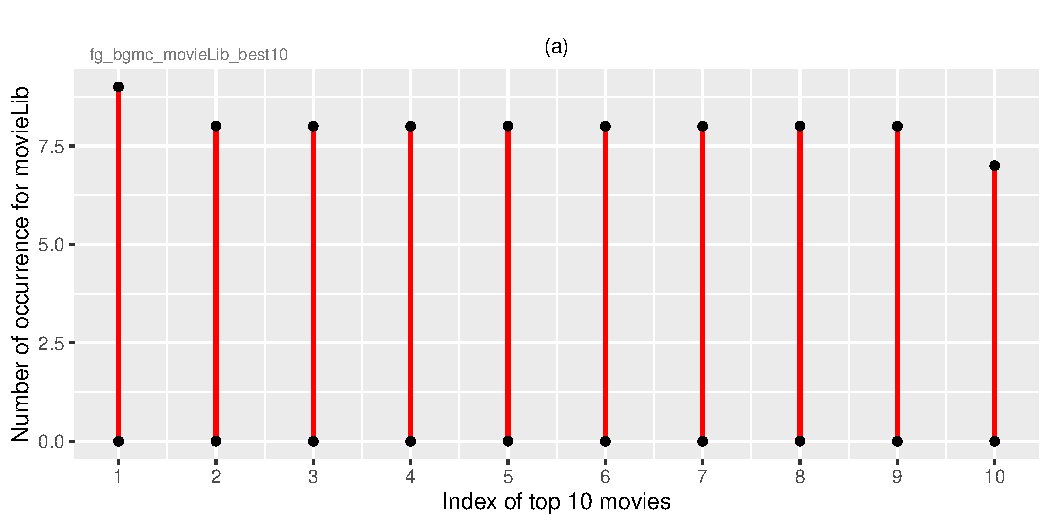
\includegraphics[width=0.48\textwidth]{_Figures/fg_bgmc_movieLib_best10}
\\[2ex]
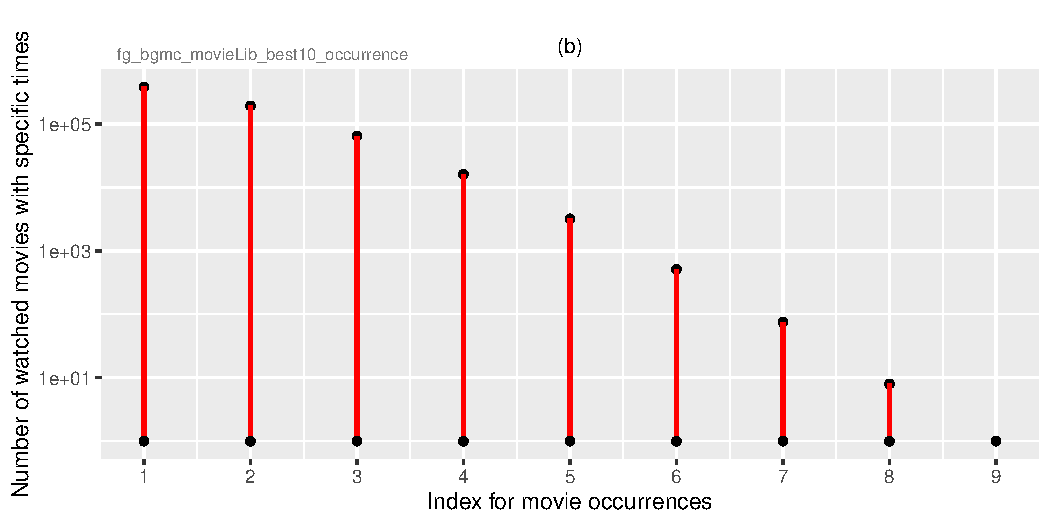
\includegraphics[width=0.48\textwidth]{_Figures/fg_bgmc_movieLib_best10_occurrence}


\caption{
These two plots relate results for the largest movie list with $2^{20}$ titles.
The plot (a) depicts the frequency of top 10 movies watched. For example, the movie with index 1 has been watched 9 times, movies with indices 2-9 have been watched 8 times, etc. 
\\
The plot (b) counts the total number of movies watched. For example, 385128 movies have been watched only once (index = 1), 75 movies have been watched 7 times (index = 7), only one movie has been watched 9 times (index = 9).
\vspace*{-3ex}
}
\label{fg_bgmc_movieLib_best10}
\end{figure}
